\section{Esqueleto funcional}\label{sec:esqueleto}

El esqueleto demuestra que la base técnica funciona: dos servicios Spring Boot 4.0.2 con Java 17 que se comunican por REST, el mecanismo elegido en el ADR-002. Los datos están en memoria; las bases de datos llegan en E3. Las instrucciones completas de ejecución están en el \texttt{README.md} del repositorio.

\subsection{Estructura del repositorio}

\begin{verbatim}
src/
  ms-usuarios/      servicio de usuarios (puerto 8081)
  ms-propuestas/    servicio de propuestas (puerto 8082)
docs/
  main.tex, sga.tex, datos.tex, referencias.bib
  secciones/        una sección del documento por archivo
  adr/              ADR-001 y ADR-002 en Markdown
  diagramas/        diagramas C4 editables (draw.io)
  figuras/          figuras del documento
  plan/             script que crea los issues
evidencias/
  levantamiento/    fotografías de las entrevistas
  fotos/            fotografías de las sesiones
  capturas/         capturas del esqueleto en ejecución
BITACORA.md
README.md
\end{verbatim}

\subsection{Servicios y comunicación}

ms-usuarios expone \texttt{GET}~\path|/api/usuarios|, con filtro opcional por rol, y \texttt{GET}~\path|/api/usuarios/{id}|, que devuelve 404 si el usuario no existe. ms-propuestas guarda cada propuesta con el id del estudiante y el del tutor. Cuando recibe \texttt{GET}~\path|/api/propuestas/{id}|, pide a ms-usuarios los datos de los dos con \texttt{RestClient} y devuelve una respuesta combinada: el título, el estado y la fecha salen de ms-propuestas, y el estudiante y el tutor, de ms-usuarios.

Los puertos se cambian con las variables \path{USUARIOS_PORT} y \path{PROPUESTAS_PORT}. ms-propuestas busca a ms-usuarios en \path{USUARIOS_URL} y espera como máximo \path{USUARIOS_TIMEOUT_MS} milisegundos (2000 por defecto). Si ms-usuarios no responde en ese tiempo, ms-propuestas contesta 503 con el mensaje \enquote{ms-usuarios no está disponible} en lugar de quedarse esperando, que es la parte de RNF-05 que ya se puede comprobar en E1.

Cada servicio trae Maven Wrapper, así que basta con tener JDK 17. Se arranca cada uno en su propia ventana:

\begin{verbatim}
cd src\ms-usuarios
.\mvnw.cmd spring-boot:run

cd src\ms-propuestas
.\mvnw.cmd spring-boot:run
\end{verbatim}

\subsection{Pruebas}

ms-usuarios tiene 4 pruebas automáticas y ms-propuestas 5; las dos suites pasan con \texttt{mvnw test}. Las de ms-propuestas usan \texttt{MockRestServiceServer} en lugar de ms-usuarios, y cubren la respuesta combinada, el tutor inexistente, el 404 y el 503 cuando ms-usuarios no contesta.

\subsection{Capturas de ejecución}

Las capturas se tomaron el sábado 21 de noviembre de 2026 entre las 00:11 y las 00:12, en la computadora de \integranteA{} (máquina Ryzen7, usuario erwin). Están sin editar en \texttt{evidencias/capturas/}.

\begin{figure}[p]
\centering
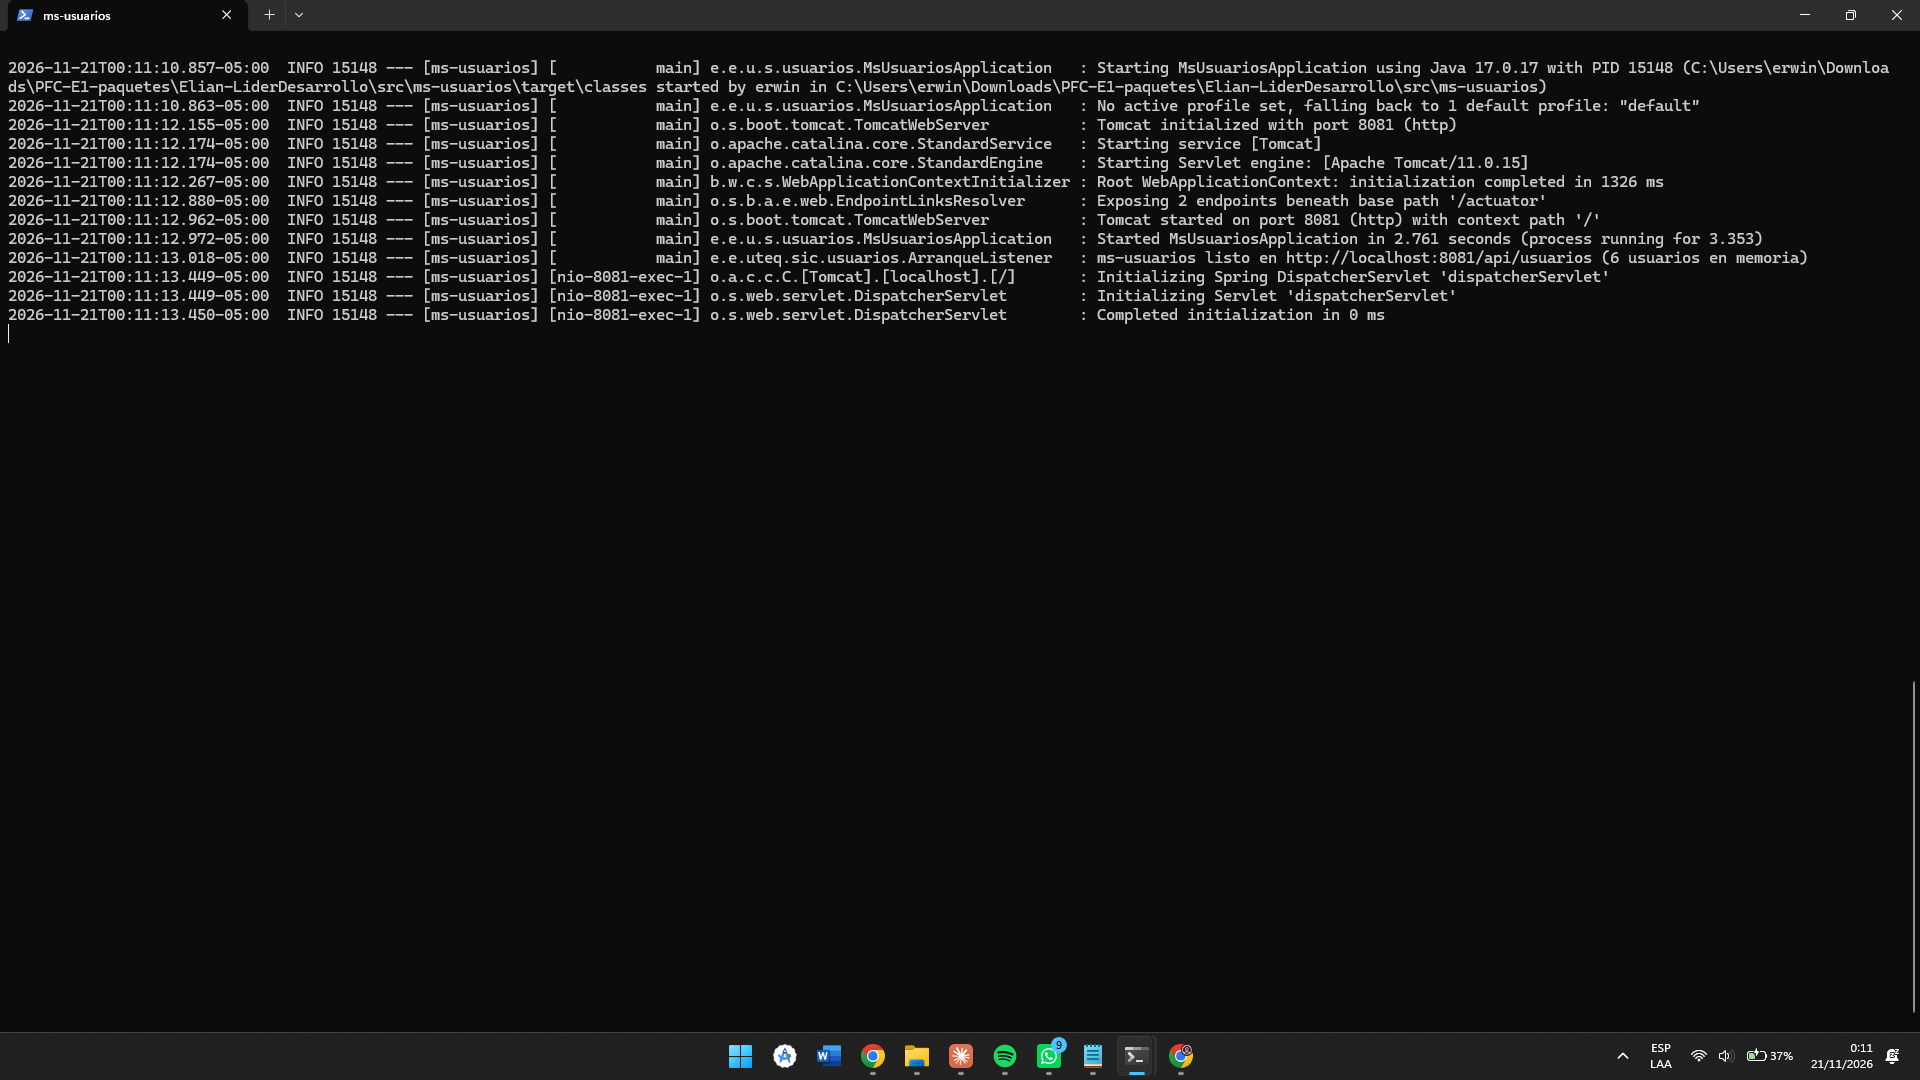
\includegraphics[width=\textwidth]{../evidencias/capturas/captura-01-ms-usuarios.png}
\caption{ms-usuarios en marcha en el puerto 8081}\label{fig:cap1}

\vspace{1cm}
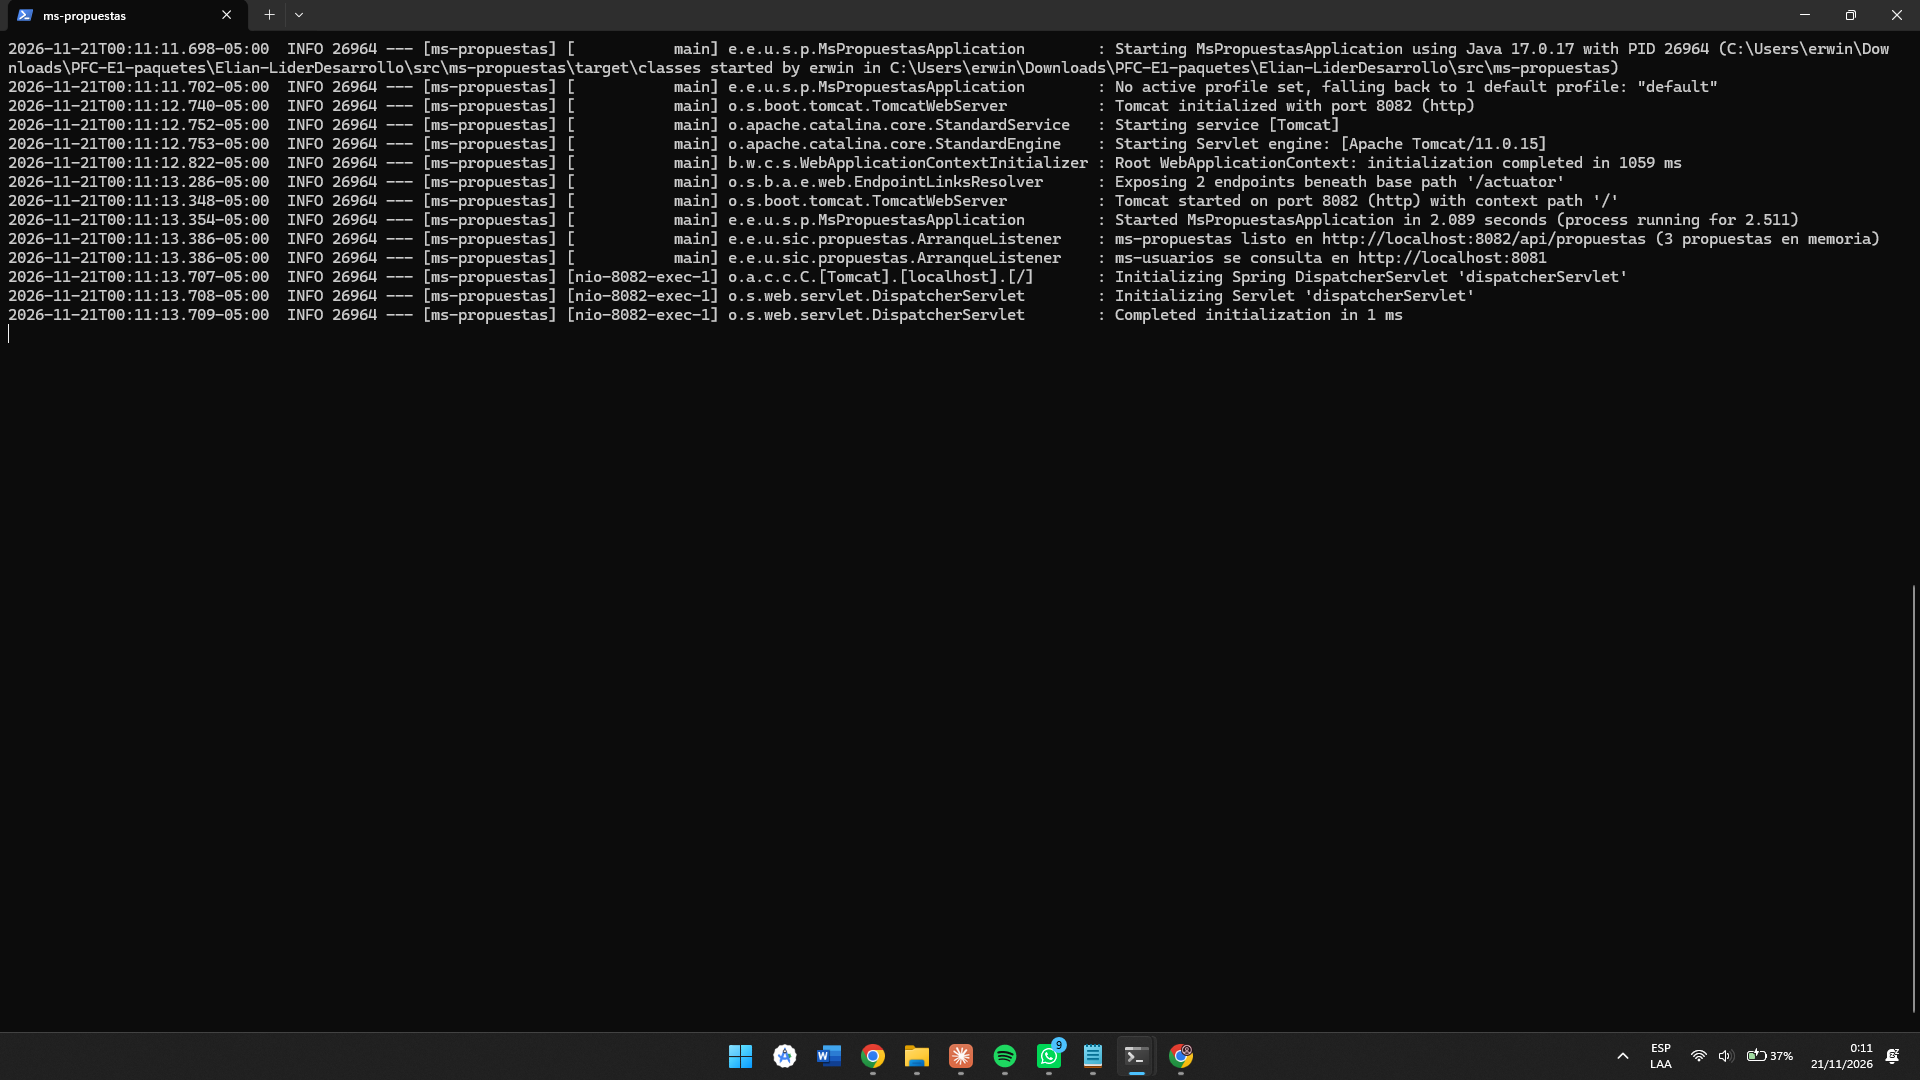
\includegraphics[width=\textwidth]{../evidencias/capturas/captura-02-ms-propuestas.png}
\caption{ms-propuestas en marcha en el puerto 8082}\label{fig:cap2}
\end{figure}

\begin{figure}[ht]
\centering
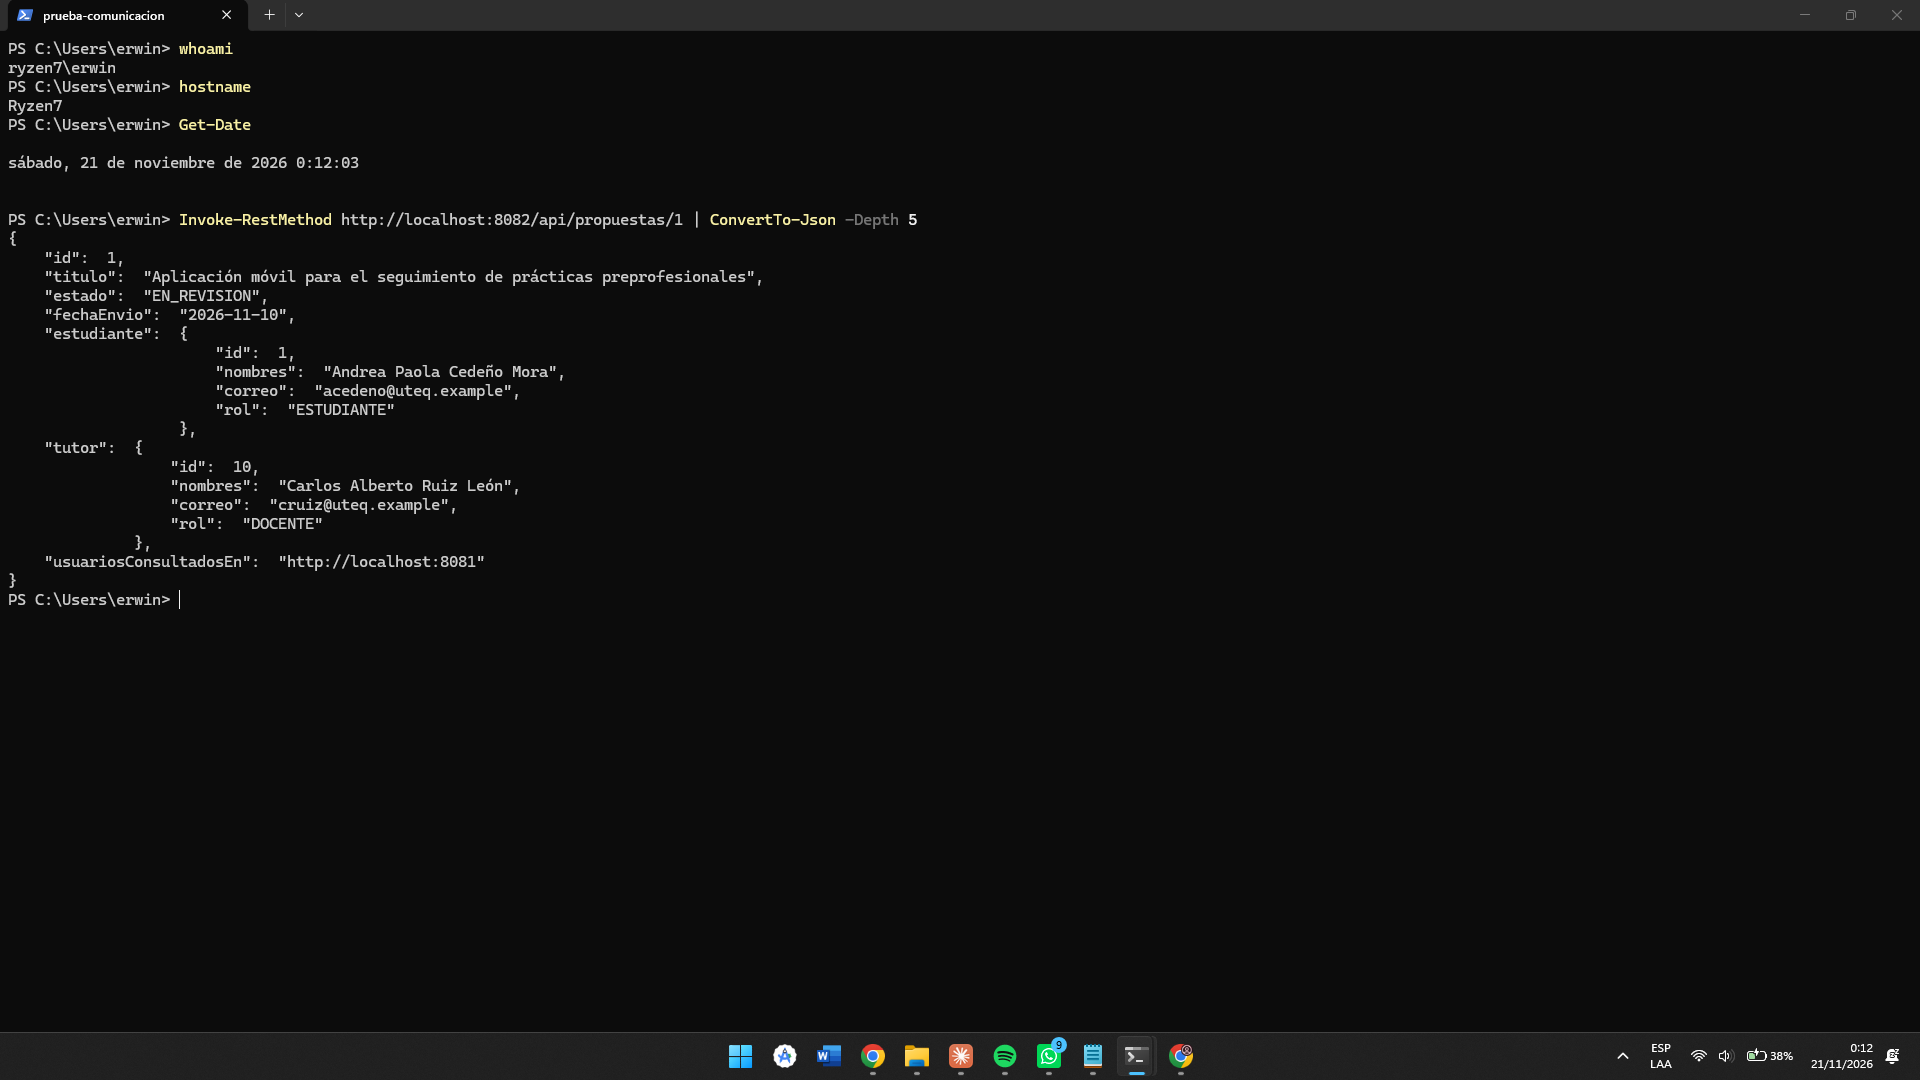
\includegraphics[width=\textwidth]{../evidencias/capturas/captura-03-comunicacion.png}
\caption{Usuario, máquina, fecha y respuesta combinada de ms-propuestas con los datos que pidió a ms-usuarios}\label{fig:cap3}
\end{figure}

% Saca aquí las capturas para que no queden después de la sección siguiente
\clearpage
